%!TEX root = main.tex
%%%%%%%%%%%%%%%%%%%%%%%%%%%%%%%%%%%%%%%%%%%%%%%%%%%%%%%%%%%%%%%%%%
\chapter{Evaluation}
\label{sec:eval}
%%%%%%%%%%%%%%%%%%%%%%%%%%%%%%%%%%%%%%%%%%%%%%%%%%%%%%%%%%%%%%%%%%

We evaluated our TorMentor design by carrying out several local
and wide-area experiments with the TorMentor prototype. Specifically,
we answer the following four research questions:

\begin{enumerate}

\item What are the effects of the privacy parameter $\varepsilon$ and
  batch size $b$ on model convergence?  (Section~\ref{eval:diffpriv})

\item What is TorMentor's overhead as compared to the baseline
  alternative? (Section~\ref{eval:overhead})
  
\item How effective are the privacy parameters $\varepsilon$ and
  minimum number of clients $k$ in defending against inversion
  attacks?  (Section~\ref{eval:inversion})
  
\item How effective is validation in defending against poisoning
  attacks, and what are the effects of its parameters?
  (Section~\ref{eval:poisoning})

\end{enumerate}

Next we describe the methodology behind our experiments and then
answer each of the questions above.

%%%%%%%%%%%%%%%%%%%%%%%%%%%%%%%%
\section{Methodology}
\label{eval:method}
%%%%%%%%%%%%%%%%%%%%%%%%%%%%%%%%%

\textbf{Credit card dataset.} In our experiments we envision multiple
credit card companies collaborating to train a better model that
predicts defaults of credit card payments. However, the information in
the dataset is private, both to the credit card companies and to their
customers. In this context, any individual company can act as the
curator, the broker is a commercial trusted service provider, and
clients are the credit card companies with private datasets.

To evaluate this use-case we used a credit card
dataset~\cite{Yeh:2009} from the \ac{UCI} machine learning
repository~\cite{Lichman:2013}. The dataset has 30,000 examples and
24 features. The features represent information about customers,
including their age, gender and education level, along with
information about the customer's payments over the last 6 months. The
dataset also contains information about whether or not the given
customer managed to pay their next credit card bill, which is used as
the prediction for the model.
 
Prior to performing the training, we normalized, permuted, and
partitioned the datasets into a 70\% training and 30\% testing shard.
For each experiment, the training set is further sub-sampled to create
a client dataset, and the testing shard is used as the
curator-provided validation set. Training error, the primary metric
used in evaluation, is calculated as the error when classifying the
entire 70\% training shard. In brokered learning, no single client
would have access to the entire training dataset, so this serves as a
hypothetical metric. \\

\noindent \textbf{Wide-area deployment on Azure.}  
We evaluated TorMentor at scale by deploying a geo-distributed set of
25 Azure virtual machines, each running in a separate data center, spanning 6
continents. Each \ac{VM} was deployed using Azure's
default Ubuntu 16.06 resource allocation. Each \ac{VM} was provisioned with
a single core Intel Xeon E5-2673 v3 2.40GHz \ac{CPU}, and 4 gigabytes of \ac{RAM}.
Tor's default \texttt{stretch} distribution was installed on each client.
We deployed the broker at our home institution as a hidden service on
Tor. The median ping latency (without using Tor) from the client
VMs to the broker was 133.9ms with a \ac{SD} of 61.9ms.
With Tor, the median ping latency increased to 715.9ms with a \ac{SD} of
181.8ms.

In our wide-area experiments we evenly distribute a varying number of
clients across the 25 VMs and measure the training error over
time. Each client joins the system with a bootstrapped sample of the
original training set (n = 21,000 and sampled with replacement), and
proceeds to participate in asynchronous model training.


%%%%%%%%%%%%%%%%%%%%%%%%%%%%%%%%
\section{Model convergence}
\label{eval:diffpriv}
%%%%%%%%%%%%%%%%%%%%%%%%%%%%%%%%%

\begin{figure}[t]
	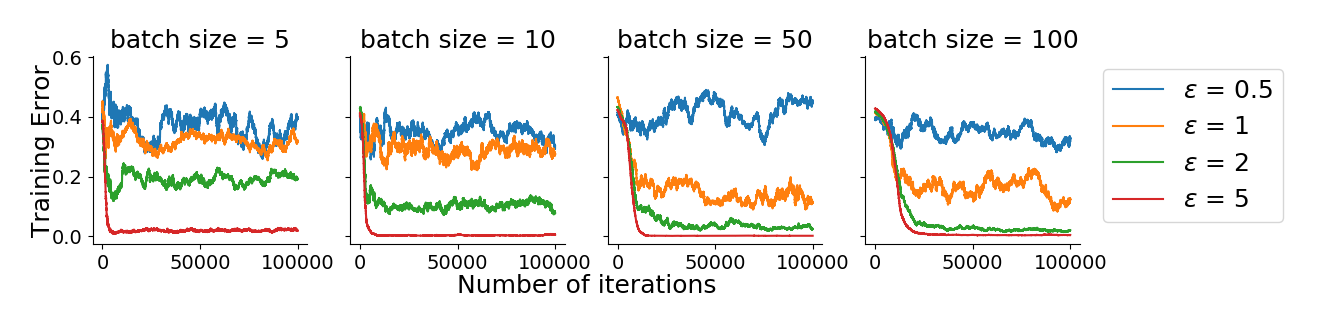
\includegraphics[width=\textwidth]{fig/giantplot}
	\caption{Effects of differential privacy and batch size on training
		loss over time. As $\varepsilon$ and $b$ decrease, model convergence
		is slower and may not be guaranteed.}
	\label{fig:bs50}
\end{figure}

We evaluate the effect of the privacy parameter $\varepsilon$ and the
batch size $b$ when performing learning over TorMentor. 
Figure~\ref{fig:bs50} shows training error over time with a single
client performing differentially private SGD~\cite{Song:2013} to
train a logistic regression model using the entire training shard.

We found that models converge faster and more reliably when the batch
size is higher and when $\varepsilon$ is higher (less privacy). These
results are expected as they are confirmations of the utility-privacy
tradeoff. In settings with a low $\varepsilon$ (more privacy) and a low
batch size we observed that the effect of differential privacy is so
strong and the magnitude of the additive noise is so large that the
model itself does not converge, rendering the output of the model
useless. Based on these results, the experiments in the remainder of the
paper use a batch size of 10.


%%%%%%%%%%%%%%%%%%%%%%%%%%%%%%%%%
\section{Scalability and overhead}
\label{eval:overhead}
%%%%%%%%%%%%%%%%%%%%%%%%%%%%%%%%%

We also evaluated TorMentor's scalability by varying the number of
participating clients. We evaluate the overhead of Tor and the
wide-area in TorMentor by running TorMentor experiments with and
without Tor. All nodes were honest, held a subsample of the original
dataset, and performed asynchronous SGD.

Figure~\ref{fig:withtor} shows that, when updating asynchronously, the
model convergences at a faster rate as we increase the number of
clients.

\begin{figure}[t]
	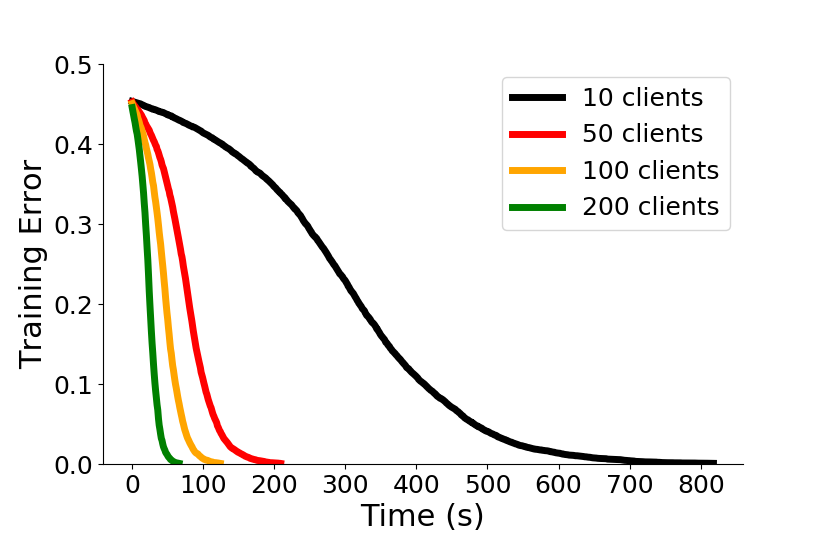
\includegraphics[width=\linewidth]{fig/withtor}
	\caption{TorMentor model convergence in deployments with 10, 50,
          100, and 200 clients.
        }
	\label{fig:withtor}
\end{figure}


We also compared the convergence time on TorMentor with a baseline
\ac{WAN} parameter server. For the WAN parameter server we used the same
clients deployment, but bypassed Tor, thereby sacrificing anonymity.

The results in Table~\ref{tab:latency} show that on average, the
overhead incurred from using Tor ranges from 5-10x. However, as the
number of clients increases, the training time in both deployments
drops, while the central deployment slows down.

\begin{table}[t]
\centering
\begin{tabular}{ c|cc }
 \hline
 \textbf{\# of Clients} & 
 \textbf{TorMentor}    & 
 \textbf{w/o Tor}  \\
 \hline
 10                    & 819 s & 210 s \\
 \hline
 50                    & 210 s  & 34 s \\
 \hline
 100                   & 135 s  & 18 s \\
 \hline
 200                   & 67 s   & 13 s \\
\end{tabular} 
\caption{Time to train the model with TorMentor, with and without Tor,
over a varying number of clients.
  \label{tab:latency}}
\end{table}

\begin{figure}[t]
	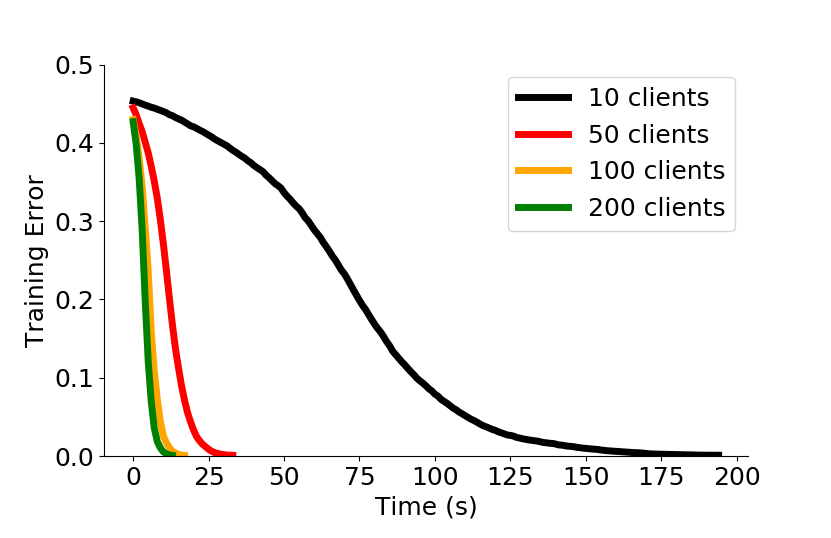
\includegraphics[width=\linewidth]{fig/withouttor}
	\caption{TorMentor without Tor model convergence in deployments with 10, 50,
          100, and 200 clients.
        %
%          \ivan{Order legend in one column: black, red, yellow, green}
        }
	\label{fig:without}
\end{figure}

\section{Inversion defenses evaluation}
\label{eval:inversion}

We first set up the inversion attack by carefully partitioning the
dataset. Of the 30,000 examples in the credit dataset, 9,000 (30\%)
examples were partitioned into $X_{test}$, a test dataset. The
remaining 21,000 examples were evenly partitioned across clients.
The victim's dataset $X_v$ was one of these partitions, with
all the $y_i$ prediction values flipped. This was done to
sufficiently separate the victim model from the globally trained
model\footnote{We originally attempted the inversion with one of the training data
shards as the victim dataset, but we found that even naively comparing
the final global model $M^*_g$ to the optimal victim model $M^*_v$
resulted in a low reconstruction error of 4.4\%. Thus, separating the
victim model in a way that makes it distinguishable is necessary.}. With
this victim dataset, a globally trained model achieved an error of
95.4\% when attempting to reconstruct the victim model, and predicting
on the test set.

With this setup we carried out the attack described in
Figure~\ref{fig:inversion-timespace}. Each attack was
executed for 4,000 gradient iterations, which was long enough for the
global model to reach convergence in the baseline case. We then
calculated the reconstruction error by comparing the resulting
inversion model to the true victim model, a model trained with only the
victim's data, by comparing predictions on the test set. That is, if
the inversion model and true victim model classify all test examples
identically, the reconstruction error is 0. The reconstruction error
would also serve as the error when an attacker uses outputs from
$\hat{M_v}$ to infer the training examples in $X_v$~\cite{Tramer:2016,
Fredrikson:2015}.

Since the inversion attack is passively performed, it is defended by a
client carefully tuning the privacy parameters $\varepsilon$ and the
minimum number of clients $k$. We evaluate the effects of these
parameters in Figures~\ref{fig:inversion-ideal}
and~\ref{fig:inversion-bystander}.

Figure~\ref{fig:inversion-ideal} shows the effect of the privacy
parameter $\varepsilon$ on the reconstruction error, as $\varepsilon$
is varied from 0.5 to 5, plotting the median and standard deviation
over 5 executions.

\begin{figure}[t]
	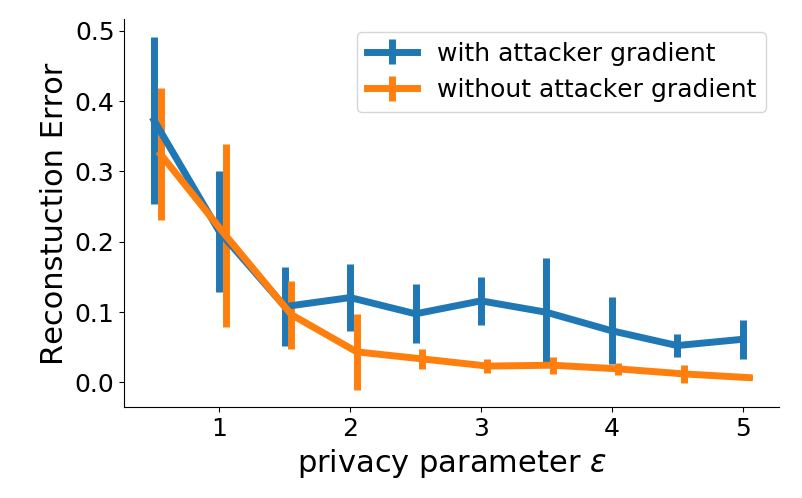
\includegraphics[width=\linewidth]{fig/inversion-ideal}
	\caption{Model agreement between victim model and inverted estimate
	in the ideal setting (Fig.~\ref{fig:inversion-timespace}), with varying $\varepsilon$.}
	\label{fig:inversion-ideal}
\end{figure}

In the baseline case the client and curator are alternating gradient
updates as in Figure~\ref{fig:inversion-timespace}, and there is no
differential privacy. As $\varepsilon$ decreases (increasing privacy),
the reconstruction error of the inversion attack increases. When
$\varepsilon = 1$, the reconstruction error is consistently 
above 10\%.

When the attacker sends a vector of zeros as their gradient update,
the inversion attack is most effective, as this completely isolates
the updates on the global model to those performed by the
victim. Figure~\ref{fig:inversion-ideal} shows the same experiment
performed when the attack contributes nothing to the global model. As
$\varepsilon$ increases beyond 2 (decreasing privacy), the attack
performed without sending any gradients consistently outperforms the
attack when performing gradient updates. This behavior, however, is
suspicious and a well designed validator would detect and blacklist
such an attacker. Therefore, this case is a worst case scenario as the
attacker must attempt to participate in the model training process.

Inversion attacks are made more difficult when randomness in the
ordering of gradient updates is increases. Two methods for increasing
this randomness include (1) adding random latencies at the broker, and 
(2) introducing bystanders: clients other than the attacker and victim.
In Figure~\ref{fig:inversion-bystander}, we evaluate both of these
methods by asynchronously training a model on TorMentor with one
victim, one attacker (using the same datasets as in 
Figure~\ref{fig:inversion-ideal}), and a varying number of bystanders.
When replying to a client response, we sample a random sleep duration
uniformly from 0-500ms at the server before returning a message.
All clients choose the same value for parameter $k$ and the actual
number of clients in the system is equal to $k$. Thus, in the framework
consisting of one victim and one attacker, the number of bystanders
equals $k-2$. 

\begin{figure}[t]
	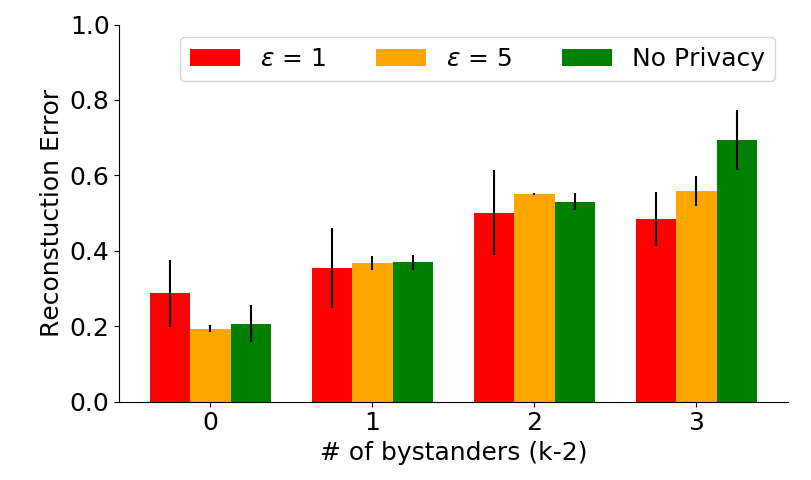
\includegraphics[width=\linewidth]{fig/inversion-bystander}
	\caption{Reconstruction error between victim model and inverted
	model estimate, with varying privacy parameters: the number of
	bystanders and the privacy parameter $\varepsilon$.
          }
	\label{fig:inversion-bystander}
\end{figure}

Introducing even just one bystander ($k=3$) into the system increases
the reconstruction error during an inversion attack from about 20\% to
40\%. As $k$ grows, a model inversion attack becomes more difficult to
mount.

Figure~\ref{fig:inversion-bystander} also illustrates that differential
privacy defends client privacy when the number of bystanders is low.
When there are no bystanders in the system, decreasing the privacy
parameter $\varepsilon$ (more private) increases the reconstruction
error. The effects of a low $\varepsilon$ value in a model inversion
setting have a higher variance than in executions with higher
$\varepsilon$ values. Another mechanism that helps to mitigate
inversion attacks is the adaptive proof of work mechanism that counters
sybils (an attacker could spawn $k-1$ sybils as an alternative way to
isolate the victim).

\section{Poisoning defenses evaluation}
\label{eval:poisoning}

We evaluate the effect of our proof of work on poisoning attacks. To
do this, we deployed TorMentor in an setting without differential
privacy or Tor in a total asynchronous setting with 8 clients. We
then varied the proportion of poisoners and the RONI threshold.
Figure~\ref{fig:poison} shows the training error for the first 250
seconds for a RONI threshold of 2\%, while varying the proportion of
poisoning attackers from 25\% to 75\%, with a validation rate of 0.1.

\begin{figure}[t]
	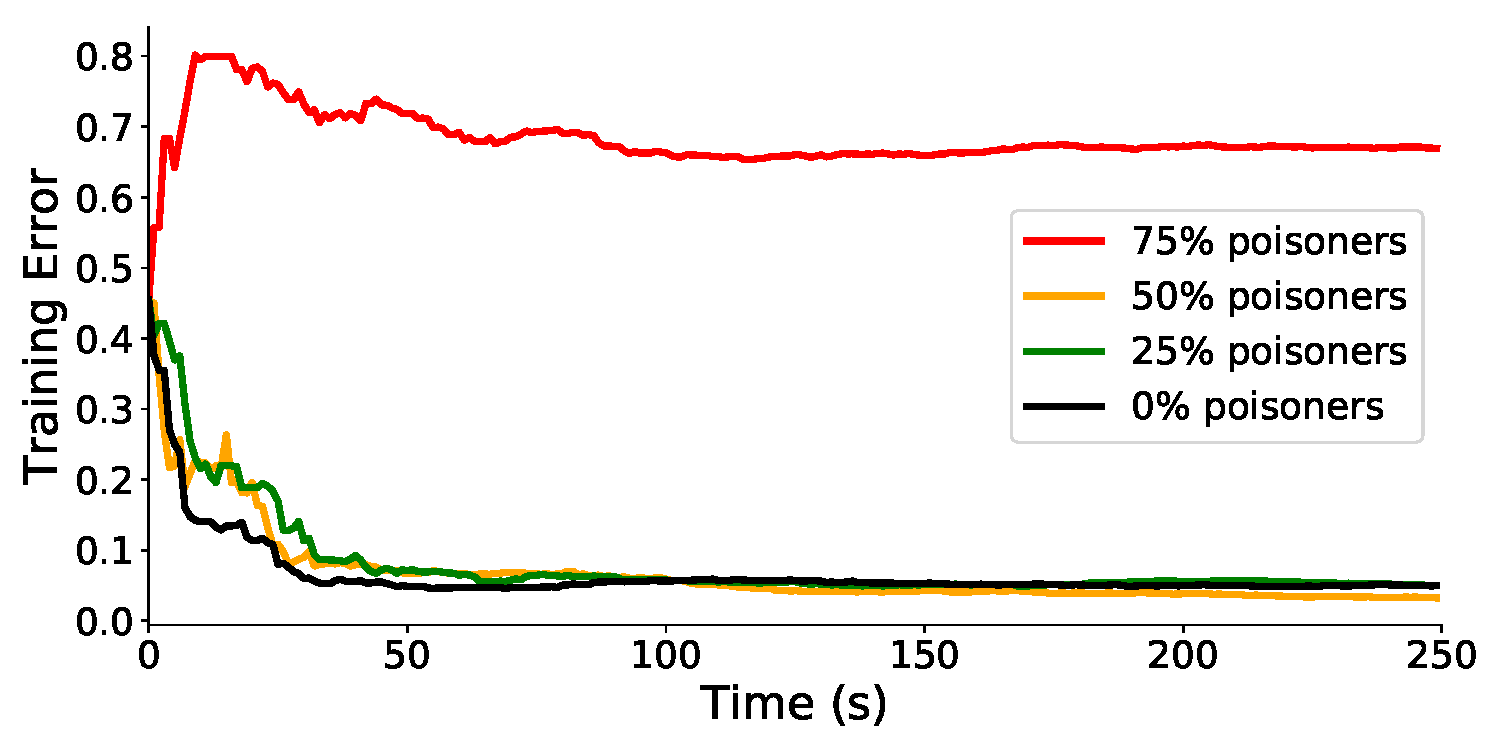
\includegraphics[width=\linewidth]{fig/poison}
	\caption{Model training loss over time, when attacked by a varying
	proportion of poisoners. RONI threshold is maintained at 2\%.}
	\label{fig:poison}
\end{figure}

As the number of poisoners increases, different effects can be
observed. When the number of poisoners is low (below 25\%), the model
still converges, albeit at a slower rate than normal. With 50\%
poisoning, the model begins to move away from the optimum, but is
successfully defended by the validator, which increases the proof of
work required for all of the poisoners within 30 seconds. From this
point, the poisoners struggle to outpace the honest nodes, and the model
continues on a path to convergence. Lastly, when the proportion of
poisoners is 75\%, the increase in proof of work is too slow to
react; the model accuracy is greatly compromised within 20 seconds and
struggles to recover.

From this evaluation, we note that, if a poisoner was able to detect
this defense, and attempt to leave and rejoin the model, an optimal
proof of work admission puzzle should require enough time such that
this strategy becomes infeasible.

\begin{figure}[t]
	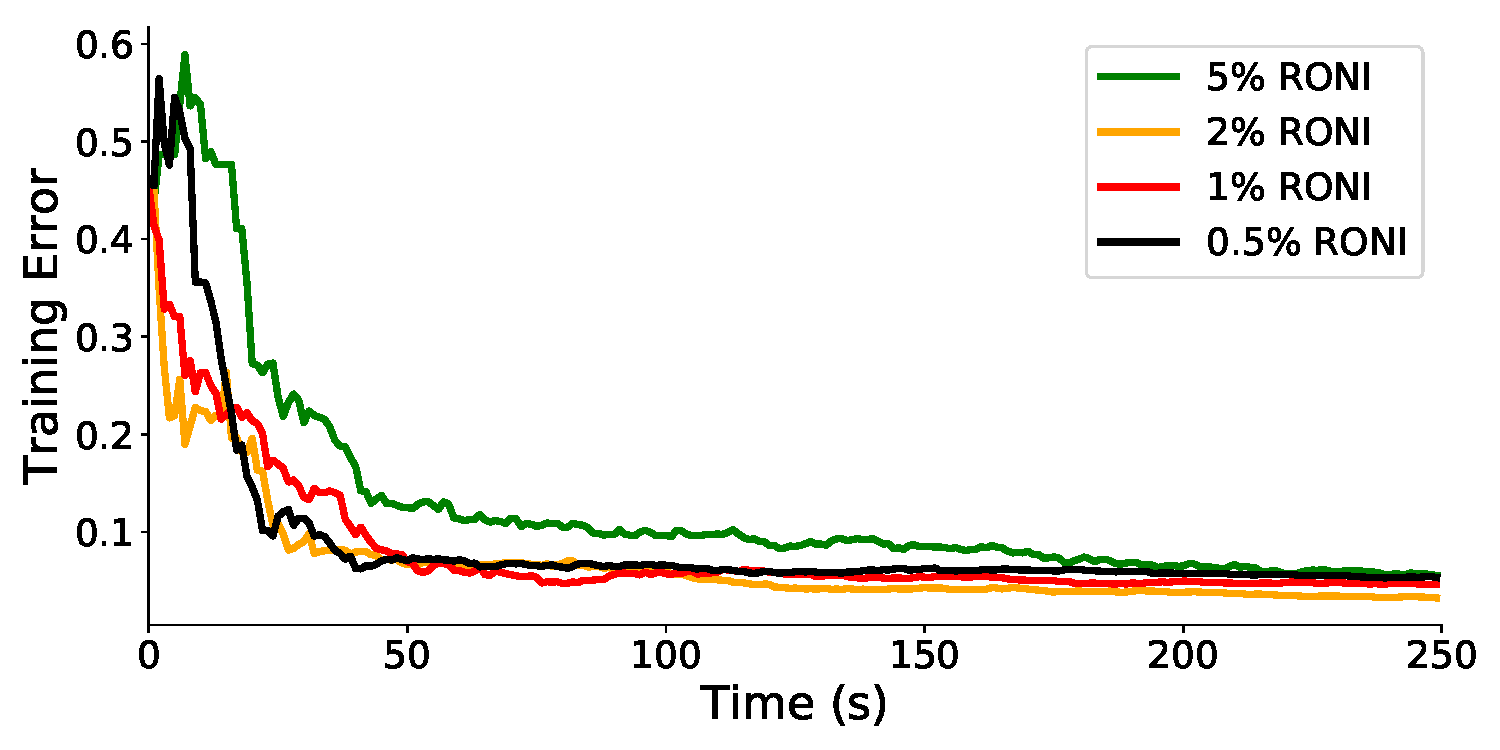
\includegraphics[width=\linewidth]{fig/thresholds}
	\caption{Model training loss over time, when attacked by 50\%
	poisoners. RONI threshold is varied from 0.5\% to 5\%. 
        }
	\label{fig:thresholds}
\end{figure}

Figure~\ref{fig:thresholds} shows the execution of model training with
50\% poisoning clients for different RONI validation thresholds. As
the threshold decreases, adversaries are removed from the system more
quickly, allowing the model to recover from the poisoning damage.

Setting the RONI threshold too low is also dangerous as it increases
the effect of false positives. In Figure~\ref{fig:thresholds}, we
observe that the model initially performs poorly, this is due to
incorrectly penalizing honest clients. The effect of a low
RONI is especially noticed in combination with differential privacy. To
confirm this, we performed two additional experiments in which the
validator had a RONI threshold of 0.5\% (the highest threshold from
Figure~\ref{fig:thresholds}), and a full set of honest clients with
differential privacy parameter $\varepsilon$ joined the model. When
$\varepsilon$ was set to 5, the model converged to an optimal point in
480 seconds. When $\varepsilon$ was set to 1, the validator flagged
all of the honest clients, and the model did not reach convergence.

The difference between model convergence, model divergence, and a
privacy violation all rely on a careful interplay between
$\varepsilon$, the minimum number of clients $k$, the RONI threshold,
the proof of work difficulty, and the anticipated attacks that
TorMentor expects to deter. Determining the optimal parameters for a
deployment depends on the anticipated workloads, data distribution, and
attack severity. Given the large scope of potential attacks and
attack scenarios in this space~\cite{Huang:2011}, we leave the
exploration of such parameter selection to future work.
